\section{RBPF-SLAM}
Once the map has been correctly generated and the simulated robot follows an adequate trajectory, it is time to enable the Rao-Blackwellized Particle Filter.\\
In the \textit{Simulation parameters} section at the top of the \textit{Main} code one can modify many parameters that have a direct impact on the result of the RBPF:

\begin{itemize}
	\item \textit{Ts}: Sampling time, by default set to happen every second.
	\item \textit{n\_cell}: sets how many centimetres a cell represents. The default is that each cell has an area of 10$cm^2$. The modification of this value should not change the structure of the code nor give any errors, but this has not been tested out yet so it is \textbf{not guaranteed} to work.
	\item \textit{NPC}: Number of particles. The more particles selected, the more accurate the occupancy grid will become, but the more computational power required for the calculations. The main advantage of the improved techniques used in this simulator for RBPF-SLAM is that the total amount of particles can be kept very low (3-6) and the results will still be fairly accurate to the reality.
	\item \textit{usable\_area}: When running the particle filter, only data in a radius of \textit{usable\_area} will be utilized, specifically, the occupancy map and the laser scan data. 
	\item \textit{sigma\_v}: Describes the standard variation of the sensor beam.
	\item R1: represents the variance matrix for the odometry. Small changes in the variance have great effects on the filter.
	\item \textit{Nsamples}: Corresponds to the number of samples to be taken when creating the Gaussian distribution. 
	\item \textit{max\_speed}: The maximum speed of the simulated robot in the vertical and horizontal axis, taking into account the size of each cell.
	\item \textit{LRS\_Sensor structure parameters}: to be set according to the laser scanner you want to model.
	\item \textit{L}: The occupancy grid is initialized to have a value of 0.5 in all of its cells. This will change on every iteration of the filter, updating the cell value to describe the probability of an exiting wall in that location.
\end{itemize}

\subsection{Filter initialisation}
The first time step of the simulation will be an initialisation of the occupancy grid map. Since we have not moved yet, the position estimate corresponds to the true value. Therefore, the generated map at this point will be very similar to the reality (except for minor laser scan variances). For this reason, the map is updated with the first scan and the particle weights and locations (which in both cases are the same for all particles) are initialised.

\subsection{RBPF simulation}
From the second iteration onwards, the particle filter will work continuously updating positions of particles and their maps. At the beginning of every iteration the new movement commands $u_t$ are calculated (based off the \textit{e} and \textit{theta} errors mentioned in section \ref{Errors}). The new true position $x_t$ is calculated assuming no errors (ideal case that does not match the reality) and 'true' scan data is obtained from the simulation.\\
The \textbf{RBPF} function is then triggered, taking all the above as arguments. After various variable initializations, the filter starts working for every particle:\\
An initial estimate of the position $x_t$ is obtained from the previous particle positions $\ddot x_{t-1}$, the movement command $u_t$ and the variance matrix $R1$ (another option would be to sample one time directly from the motion model). An estimated laser scan is obtained from teh estimated position and the last iteration of the occupancy grid map for that particle via the \textbf{Measurement\_Estimate\_From\_Grid} method. Before the ICP (scan-matching) algorithm can be applied, the 'true'scan $y$ and the estimated one $y_h$ have to be pre-processed. Since the laser data is in radial form (laser angle and distance) it will be easier to match one-to-one scan. To do so, all scans that have a distance bigger than \textit{usable\_area} will be depreciated. This helps computational-wise and focuses only on scans that come from areas of the map that are closer to the robot and, thus, are more reliable. Theoretically, those scans that are neglected in $y$ should also be in $y_h$, and vice versa. In reality, sometimes they do not and those scans that mismatch because of this will also be neglected to avoid errors in the ICP algorithm. Finally, the scans are converted to Cartesian space and put in the World frame and the initial estimate position $x_t$ is also included in the point cloud for reasons described below.\\
The ICP algorithm is run between both datasets ($y$ and $y_h$). If the ICP reports a failure or generates translational or rotational matrices which are erroneous, the final position estimate of the particle $\ddot x_t$ will be equal to the initial estimate $x_t$ that simply came from the odometry distribution. In the cases where the ICP succeeds, a translational $TT$ and rotational $TR$ matrix are returned; these represent the movement the estimated laser scan data $y_h$ has to follow to converge to the 'true' scan data $y$. 

\begin{wrapfigure}{L}{0.4\textwidth}
	\renewcommand\figurename{Fig.}
	\begin{center}
		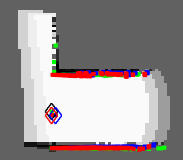
\includegraphics[width=0.38\textwidth]{figures/path-image}
	\end{center}
	\caption{Different position estimates and scans: true, before ICP and after}
\end{wrapfigure}

The trick here is that the ICP also returns the rotated data (which should, in most cases, have converged), and since the initial estimated position was included in the dataset, a better estimate of the position $\dot x_t$ thanks to scan-matching is already derived (the $\theta$ value will remain the same as the one previously estimated). This is automatically visualized through a figure which has, in the background, a grey-scaled image of the occupancy grid map up until that point, the diamond shaped points that represent the positions (black: true position, blue: initial estimate, red: new estimated position after scan-matcher). In the same manner, the laser scans are represented where green is the true scan, blue is the scan obtained from the previous occupancy map and an initial estimate, and red would be the converged scan.

The next step is obtaining samples $x_j$ to create the Gaussian distribution. These samples are randomly selected around $\dot x_t$ and will be used to evaluate the target proposal consisting
of the odometry distribution $p(x_j|x_{t-1}^{(i)}, u_t)$ and the observation likelihood $p(z_t| x_j, m^{(i)})$. The former is derived by means of the function \textbf{Motion\_Model\_Velocity} which returns the probability of a final position given an initial one and a movement command. The latter is obtained via a scan matching procedure. The approach selected is a point-to-point comparison between the true scan and the scan obtained from the current map for that sample. Both distributions are then multiplied point-wise to obtain the target proposal $\tau$.\\
The weighing factor $\eta^{(i)}$, the Gaussian mean $\mu_t^{(i)}$ and the covariance $\Sigma_t^{(i)}$ are calculated. The particle weights are also updated. Additionally, the final position estimate for that particle $\ddot x_t$ is sampled from the Gaussian. Finally, the map for that particle is updated given the final estimated position $\dot x_t$ and the true laser scan.\\
To check if a resample is necessary, the weights are normalized and $N_eff$ is derived. In the case that this value is smaller than a given percentage of the total amount of particles, a resampling step must be taken. If not, no further steps are required.



